\documentclass{article}
\usepackage{hyperref}
\hypersetup{
    pdftitle={Project Circinus v1.2.4},
    pdfsubject={Spherical trigonometry, and a whole load of baloney},
    pdfauthor={qihao}
}

\usepackage[utf8]{inputenc}
\usepackage[a4paper,margin=0.75in, footnotesep=0.25in]{geometry}
\usepackage[bottom]{footmisc}

\usepackage{xifthen}

\usepackage{parskip}
\usepackage{varwidth}
\usepackage{exercise}
\usepackage{enumitem}

\usepackage{amsmath}
\usepackage{amssymb}
\usepackage{rotating}
\usepackage{graphicx}
\usepackage{pgfplots}
\pgfplotsset{compat=1.18}
\usepackage{tkz-euclide}
\usetikzlibrary{positioning,angles,calc,quotes,intersections,decorations.text,arrows,pgfplots.fillbetween}

\linespread{1.05}

%% 
%%  Exercise customization
%%
\renewcommand{\ExerciseHeader}{%
    \textbf{\ExerciseName\ \ExerciseHeaderNB\ ---}%
}%
\renewcommand{\AnswerHeader}{%
    \smallskip\textbf{Solution: }%
}%
\renewcommand{\ExerciseListHeader}{%
    \textbf{\ExerciseName\ \ExerciseHeaderNB\ --- }%
}%

%%
%%  Angle formatting commands
%%
\newcommand{\degree}{{}^{\circ}}
\newcommand{\sexg}[3]{%
    \ifthenelse{\isempty{#2}}%
        {{#1}\degree}%
        {\ifthenelse{\isempty{#3}}%
            {{#1}\degree {#2}'}%
            {{#1}\degree {#2}' {#3}''}%
        }%
}%
\newcommand{\hms}[3]{%
    \ifthenelse{\isempty{#2}}%
        {{#1}^{\mathrm{h}}}%
        {\ifthenelse{\isempty{#3}}%
            {{#1}^{\mathrm{h}} {#2}^{\mathrm{m}}}%
            {{#1}^{\mathrm{h}} {#2}^{\mathrm{m}} {#3}^{\mathrm{s}}}%
        }%
}%
\newcommand{\h}{{}^\mathrm{h}}
\newcommand{\RA}{\mathrm{RA}}
\newcommand{\HA}{\mathrm{HA}}
\newcommand{\EOT}{\mathrm{EOT}}

%%
%%  Layout commands
%%  
\newcommand{\flipanswer}[1]{\rotatebox[origin=c]{180}{\footnotesize #1}}

\setlength{\fboxsep}{0.75em}
\setlength{\fboxrule}{0.75pt}
\newcommand{\boxedtext}[1]{%
    \smallskip%
    \fbox{\begin{varwidth}{\textwidth}{#1}\end{varwidth}}%
    \smallskip%
}
\newcommand{\smallboxedtext}[1]{%
    \smallskip%
    \begin{center}\framebox{$\quad${#1}$\quad$}\end{center}%
    \smallskip%
}
\newcommand{\crule}{%
    \smallskip%
    \begin{center}\noindent\rule{0.5\textwidth}{0.4pt}\end{center}%
    \smallskip%
}

%%
%%  Counters
%%
\numberwithin{equation}{section}

\title{Project Circinus}
\author{qihao}
\date{}

\begin{document}

\maketitle

\section{An Attempt at History}
\subsection{The Invention of Geometry}
At least a decade ago, a wise man by the name of Euclid wrote a treatise called \textit{The Elements}. As the name clearly suggests, it was a book of mathematics that contained cool stuff about geometry. There are many things inside, but let us concern ourselves only with Euclid's fifth postulate:

\begin{figure}[h]
    \centering
    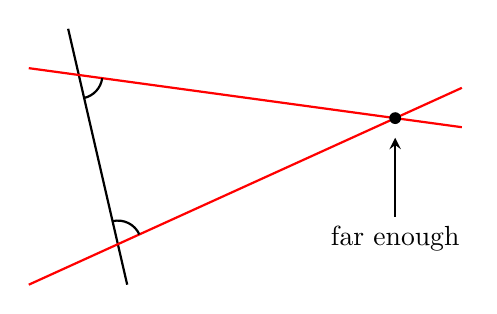
\begin{tikzpicture}[>=stealth]
        \draw[thick,black,name path=base] (0,1.5) -- (0.75,-1.75);
        \draw[thick,red,name path=line1] (-0.5,1) -- (5,0.25);
        \draw[thick,red,name path=line2] (-0.5,-1.75) -- (5,0.75);
        \fill[name intersections={of=line1 and line2, by={X}}] (X) circle (0.075);
        \draw[thick,->] ($(X)-(0,1.25)$) coordinate (Xl) -- ($(X)-(0,0.25)$);
        \node [below] at (Xl) {far enough};
        \path[name intersections={of=line1 and base, by=Y}];
        \path[name intersections={of=line2 and base, by=Z}];
        \draw pic[draw=black,thick,angle eccentricity=1.2,angle radius=0.3cm] {angle=Z--Y--X};
        \draw pic[draw=black,thick,angle eccentricity=1.2,angle radius=0.3cm] {angle=X--Z--Y};
    \end{tikzpicture}
    \caption{Postulate No. 5}
\end{figure}

\boxedtext{Two lines that intersect a third line such that their inner angles is \textbf{less than 180$\degree{}$} will eventually intersect each other on that side if extended far enough.}

I'm sure you're aware that parallel lines never meet. This \textit{very important fact} follows from the fifth postulate. Quite a few mathematicians were convinced that this was derivable from the previous first four axioms\footnote{Disclaimer: It was not}. This went on for a couple hundred years.

\subsection{The Invention of Curvature}
Back in Euclid's day, balloons hadn't existed yet. It wasn't until balloons were commercially available that geometers could start doing problem sets on curved surfaces. This made it much more entertaining because there was an additional element of suspense, as you never knew when they would pop\footnote{I didn't study history but I think this is true}.

However, these party geometers soon realized that balloons violated their beloved fifth axiom. That really \textit{burst} their bubble.

\begin{Exercise}
Imagine yourself as a party geometer. Try drawing a triangle and a pair of parallel lines on an inflated balloon. What do you observe?
\end{Exercise}
\medskip

The fifth postulate is very important in its own right; it lays down the groundwork for defining \textit{Euclidean geometry}. This is arguably the most important geometry because it is applicable to daily life and Minecraft.

\subsection{If Geometry was so good, why isn't there a Geometry 2?}
In fact, geometries come in all sorts of shapes and sizes. Could you invent your own geometry? Probably. Would it be useful? Probably not.

Different geometries describe different spaces. As an illustration, lets look at a Non-Euclidean geometry. A simple and commonly used one is the taxicab geometry.
\medskip

\begin{figure}[h]
    \centering
    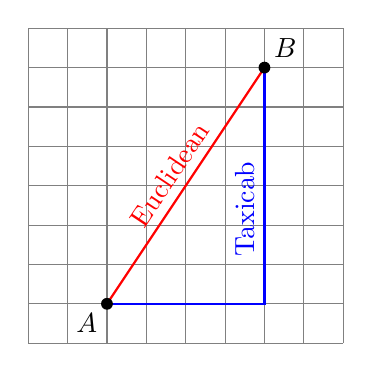
\begin{tikzpicture}
        \draw[gray,thin,step=0.5] (0,0) grid (4,4);
        \coordinate (A) at (1,0.5);
        \coordinate (B) at (3,3.5);
        \draw[thick,red] (A) -- (B) node[midway,above,sloped] {Euclidean};
        \draw[thick,blue] (A) -- (3,0.5) -- (B) node[pos=0.4,above,sloped] {Taxicab};
        \fill[black] (A) circle (0.075) node[anchor=north east] {$A$};
        \fill[black] (B) circle (0.075) node[anchor=south west] {$B$};
    \end{tikzpicture}
    \caption{Taxicab Geometry}
    \label{fig:taxicab}
\end{figure}

In ordinary  geometry, the distance between two points $A$ and $B$ is given by
\begin{equation*}
    d = \sqrt{(\Delta x)^2 + (\Delta y)^2}
\end{equation*}
\medskip
In the taxicab geometry (Fig.\;\ref{fig:taxicab}), the distance is measured only along the vertical and horizontal axes
\begin{equation*}
    d = |\Delta x| + |\Delta y|
\end{equation*}

Using a different geometry can offer another way of looking at the same space. They prescribe the mathematical lens through which we describe shapes and their spatial relationships. Astrophysics employs a bunch of them -- you can find hyperbolic and elliptical geometries in cosmology. Einstein's famous General Relativity uses Riemannian geometry, which is just a jumble of geometries on steroids.

Let us declare war against Euclid and commit sacrilege upon his fifth postulate. Henceforth, we shall enter the world of \textit{spherical geometry} -- a simplified case of elliptical geometry. As heretics, we shall bathe in the glory of parallel lines that \textbf{can} intersect.

\section{Spherical Geometry}
It is now time to get out your balloons (only spherical ones allowed) and throw away your flat paper! I highly recommend carrying a packet of balloons everywhere in case you encounter an astrophysics question in the wild.

We will be working with the \textbf{2-D} surface of a ball\footnote{Strictly speaking, a sphere is the 2-D surface $x^2+y^2+z^2=r^2$, whereas a ball is a 3-D object formed by the points $x^2+y^2+z^2 \leq r^2$. This describes a \textit{closed} ball, and for \textit{open} balls the inequality is strict}. As with the taxicab example, we can interpret this same space in two different ways:
\begin{itemize}
    \item A 2-D surface embedded in a 3-D space. This is useful for illustrating concepts as we can consider points inside the ball.
    \item Strictly a 2-D surface. Imagine yourself as an ant crawling on a ball -- there is no up or down, only the seemingly repeating surface to which you are confined to roam for eternity, a truly Sisyphean and 2-D surface.
\end{itemize}

Before we take the train into spherical trigonometry town, let us clarify some terms first.

\begin{figure}[h]
    \centering
    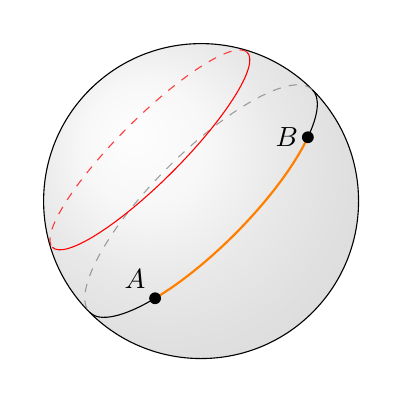
\begin{tikzpicture}[rotate=45]
        \shade[ball color=gray!40,opacity=0.2] (0,0) circle (2);
        \draw (0,0) circle (2);
        % great circle
        \draw (-2,0) arc (180:230:2 and 0.6);
        \draw (2,0) arc (0:-40:2 and 0.6);
        \draw[orange,thick] (230:2 and 0.6) arc (230:320:2 and 0.6);
        \fill[black] (230:2 and 0.6) circle (0.075) node[anchor=south east] {$A$};
        \fill[black] (320:2 and 0.6) circle (0.075) node[anchor=east] {$B$};
        \draw[dashed,opacity=0.75,gray] (2,0) arc (0:180:2 and 0.6);
        % small circle
        \draw[red] (-1.75,0.92) arc (180:360:1.75 and 0.4);
        \draw[red,opacity=0.75,dashed] (1.75,0.92) arc (0:180:1.75 and 0.4);
    \end{tikzpicture}
    \caption{\texttt{graphics design is my passion}}
    \label{fig:great_circle}
\end{figure}

\subsection{Terminology}
When we talk about lines in spherical geometry, we are actually referring to a \textit{great circle} (Fig.\;\ref{fig:great_circle} - in black).
\begin{itemize}
    \item Great circles are the largest circles possible on the sphere
    \begin{itemize}
        \item (Equivalently) The plane containing a great circle also contains the diameter of the sphere
        \item (Equivalently) The center of a great circle coincides with the center of the sphere
    \end{itemize}
    \item Two great circles will intersect each other at two \textit{antipodal} points (opposite ends of the sphere)
    \item Any line that is not a great circle is a \textit{small circle} (red). You should never be doing calculations on one of these!
    \item A section of a line is an \textit{arc} (orange)
\end{itemize}
These great circles are the analogue of straight lines from Euclidean geometry. Just like straight lines, an arc of a great circle will always be the shortest path\footnote{If you want street cred, call these \textit{geodesics}} between two points. The definition of the distance between these points is the length of this arc.

\begin{Exercise}
For any two points, is there always a unique arc connecting them? What about the distance between them?
\end{Exercise}
\begin{Answer}
Two points will only be joined by one unique great circle, split into two arcs -- one short and one long. The exception are antipodal points, which have an infinite number of lines connecting them. In any case, the length is always well defined.
\end{Answer}
\medskip


A spherical triangle is a triangle (surprise!) composed of three arcs (Fig.\;\ref{fig:spherical_triangle}). It is a good time as ever to tell you now that distances are measured in \textbf{angular units}. However, these `length' angles ($a, b, c$) are different from the `angle' angles between arcs ($A, B, C$). These `length' angles are angles along the great circles, and can be thought of as the angle subtended by the arc from the center of the sphere ($\theta_b$). Triangles with a $90\degree$ angle are \textit{right spherical triangles} and those with a $90\degree$ edge are \textit{quadrantal triangles}.

\begin{figure}[h]
    \centering
    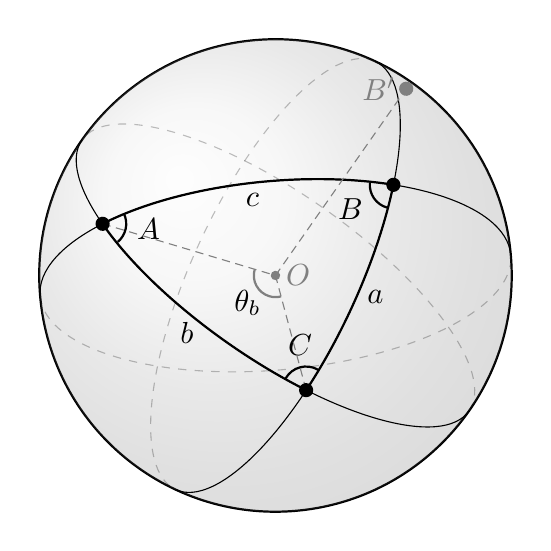
\begin{tikzpicture}[rotate=5,scale=1.5,every node/.style={scale=1.1}]
        \coordinate (O) at (0,0);
        % Sphere
        \draw[thick] (O) circle (2);
        \shade[ball color=gray!40,opacity=0.2] (O) circle (2);
        % Arcs
        \draw[name path=arc1] (2,0) arc (0:180:2 and 0.8) node[below,pos=0.52] {$c$};
        \draw[dashed,opacity=0.25] (-2,0) arc (180:360:2 and 0.8);
        \draw[name path=arc2,rotate=60] (-2,0) arc (180:360:2 and 0.7) node[right,pos=0.52] {$a$};
        \draw[dashed,opacity=0.25,rotate=60] (2,0) arc (0:180:2 and 0.7);
        \draw[name path=arc3,rotate=140] (2,0) arc (0:180:2 and 0.7) node[below,pos=0.43] {$b$};
        \draw[dashed,opacity=0.25,rotate=140] (-2,0) arc (180:360:2 and 0.7);
        % Vertices
        \path[name intersections={of=arc1 and arc3,by=A}]; 
        \path[name intersections={of=arc1 and arc2,by=B}];
        \path[name intersections={of=arc3 and arc2,by=C}];
        % Triangle
        \draw[thick] (58:2 and 0.8) arc (58:135:2 and 0.8);
        \draw[thick,rotate=60] (247:2 and 0.7) arc (247:304:2 and 0.7);
        \draw[thick,rotate=140] (44:2 and 0.7) arc (44:113:2 and 0.7);
        % Angles
        \draw[thick] ([shift=(305:0.2)]A) arc (305:380:0.2) node[pos=0.5,right] {$A$};
        \draw[thick] ([shift=(170:0.2)]B) arc (170:250:0.2) node[pos=0.5,below left=-4pt and 0pt] {$B$};
        \draw[thick] ([shift=(55:0.2)]C) arc (55:145:0.2) node[pos=0.5,above] {$C$};
        % Subtended angle
        \draw[gray,densely dashed] (A) -- (O) -- (C);
        \draw[thick] pic[draw=gray,angle eccentricity=1.2,angle radius=0.25cm] {angle=A--O--C};
        \node [below left=2pt] at (O) {$\theta_b$};
        \fill[gray] (O) circle (0.04) node[right] {$O$};
        % Pole of AC
        \draw[gray, densely dashed] (0,0) -- (50:1.93);
        \fill[gray] (50:1.93) circle (0.06) node[left] {$B'$};
        % Draw vertices on top
        \fill (A) circle (0.06);
        \fill (B) circle (0.06);
        \fill (C) circle (0.06);
    \end{tikzpicture}
    \caption{I'm not gonna draw this again it was very painful}
    \label{fig:spherical_triangle}
\end{figure}

Having desecrated the domain of Euclidean geometry we are all so accustomed to, we will also need to give up some familiar properties:
\smallboxedtext{The angles in a spherical triangle \textbf{do not add up to $180\degree$}}

\subsection{I hope you like math}
Unfortunately, you can no longer measure angles with a protractor and lie to yourself that the diagram is drawn to scale. The only measuring tool we have now is called mathematics, which provides a way to relate angles to each other.

\subsubsection{Doctors Hate Him! Save Time Using This ONE WEIRD TRICK!!}
If you think about it, having 360 degrees to a circle is quite weird. Being familiar with base 10, a relic such as the sexagesimal system (base 60) is pretty wack, but it all boils down to culture and society. We think that the decimal system makes sense because we have 10 fingers. In French and many African dialects, they use the vigesimal system (base 20) because they remembered they have toes\footnote{I am not an anthropologist nor a linguist}. The Oksapmin, with their massive brain, have adopted a base 27 system that utilizes their fingers, arms and face.

The Babylonians probably didn't use body parts to count to 60, but nevertheless, this was the system that mathematics inherited for angles. Just like how we have tenths and hundredths in the decimal system, base 60 has arcminutes and arcseconds. 1 degree is 60 arcminutes (denoted 60') and an arcminute is 60 arcseconds (60''). We will be using these fractional parts very often.

At this juncture, if you don't know how to use the sexagesimal (that $\degree$'\," thing) button on your calculators, I suggest you learn how to use it. You \textit{could} manually divide by 60 each time, but you \textit{should} find better things to do with your time.

Also, \textbf{\textcolor{red}{always check that you are using the correct angular units}}. Most, if not all, of the time you will be working with degrees. I'm not sure why you would ever use radians in spherical trigonometry. I'm not very sure what a grad does, but you won't use it either.

\subsubsection{Basics}
The spherical sine law is as simple as it gets:
\begin{equation}
    \frac{\sin a}{\sin A} = \frac{\sin b}{\sin B} = \frac{\sin c}{\sin C}
\end{equation}
Do note that when using the sine law can give you \textbf{ambiguous answers} since $\sin(\theta) = \sin(180\degree - \theta)$. When applying these to astronomy questions, there will usually be contextual knowledge to eliminate one answer.

\crule

The spherical cosine law is not as simple:
\begin{equation}
\label{eqn:cosine_law}
    \cos a = \cos b \cos c + \sin b \sin c \cos A
\end{equation}
I suggest you remember this using the relative positions of the quantities, as the parameters will almost never be spoon-fed to you in terms of these letters. It is easier to think of the cosine law as expressing the cosine of an edge in terms of its adjacent edges and the opposite angle. Master this spatial memorization and spherical triangles will literally solve themselves in terror of your prowess.

\begin{Exercise}
Find $b$ and $C$, given $A=\sexg{78}{2}{}$, $B=\sexg{35.217}{}{}$, $a=\sexg{23}{14}{12.17}$, $c=\sexg{22}{10}{5.08}$. Do the angles add up to $180\degree$?
\end{Exercise}
\begin{Answer}
\flipanswer{$b=\sexg{13}{26}{54} \quad C=\sexg{69}{19}{34}$}
\end{Answer}
%%
\begin{Exercise}
Solve the spherical triangle with $A=\sexg{53}{14}{7.2}$, $b=\sexg{24}{15}{31}$ and $c=\sexg{29}{17}{58.3}$.
\end{Exercise}
\begin{Answer}
\flipanswer{$a=\sexg{23}{44}{9} \quad B=\sexg{54}{51}{16} \quad C=\sexg{76}{53}{50}$}
\end{Answer}

\subsubsection{Acidics}
Theoretically, you now possess the ability to solve any spherical problem thrown at you. The cold hard truth however, is that you will give up after being repeatedly bludgeoned with simultaneous trigonometric equations, and succumb to dehydration from your endless stream of tears.

\begin{figure}[h]
    \centering
    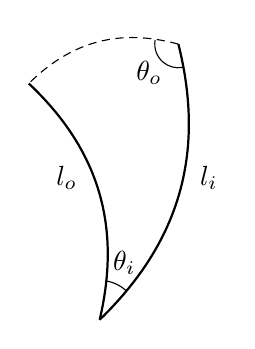
\begin{tikzpicture}
        \coordinate (A) at (0.7, 1.7);
        \coordinate (B) at (-1.2, 1.2);
        \coordinate (C) at (-0.3, -1.8);
        \draw[densely dashed] (A) to[bend right] (B);
        \draw ([shift=(47:0.5)]C) arc (47:80:0.5) node[black,pos=0.5,above right=0pt and -5pt] {$\theta_i$};
        \draw ([shift=(170:0.3)]A) arc (170:280:0.3) node[black,pos=0.5,below left=-5pt] {$\theta_o$};
        \draw[thick] (B) to[bend left=30] (C) node[black,pos=0.5,left=13pt] {$l_o$};
        \draw[thick] (A) to[bend left=30] (C) node[black,pos=0.5,right=24pt] {$l_i$};
    \end{tikzpicture}
    \caption{Geometer's deformed cheese slice}
    \label{fig:triangle}
\end{figure}

A particularly useful equation for astronomy is the cotangent four-part formula, which can be derived from the sine double-two-part and cosine three-part formulae above. It's not particularly difficult, but the derivation is detailed in Appendix \ref{app:derivations} should you need some help. It is easier to think of the formula in terms of outer/inner angles or edges as shown in Fig.\;\ref{fig:triangle}:
\begin{equation}
    \label{eqn:cotangent_four_part}
    \cos l_i \cos \theta_i = \cot l_o \sin l_i - \cot \theta_o \sin \theta_i
\end{equation}

It is highly recommended that you devise some mnemonic instead of memorizing the formula as is. I have heard of a brilliant example from a wise intellectual\footnote{Me, c. 2017}. However, on the advice of my legal counsel, I should refrain from putting it in print.

\crule

Any spherical triangle has its own fraternal twin called a \textit{polar triangle}. For brevity, we denote the vertices and edges of the polar triangle with $()'$. Drawing a polar triangle is pretty simple:
\begin{enumerate}
    \item Pick a vertex of the triangle (e.g. $B$ in Fig.\;\ref{fig:spherical_triangle}) and find its opposite edge ($b$)
    \item Find the great circle containing this arc
    \item From the center of this great circle, draw the perpendicular towards the surface of the hemisphere containing $B$. This is the pole of $B$ ($B'$).
    \item Repeat the above for the other vertices and connect them to form the polar triangle $A'B'C'$
\end{enumerate}

An interesting property (which are outside the scope of these notes\footnote{I got lazy and it was never useful anyways}) is that the length and edges of the polar triangle are \textit{supplementary} to those of the original triangle
\medskip
\begin{center}
\begin{tabular*}{0.6\textwidth}{@{\extracolsep{\fill} }ccc}
    $A' = 180\degree - A$ & $B' = 180\degree - B$ & $C' = 180\degree - C$ \\
    $a' = 180\degree - a$ & $b' = 180\degree - b$ & $c' = 180\degree - c$
\end{tabular*}
\end{center}
\medskip
Revolutionary! Not quite. This does, however, give us the supplemental cosine law which is just Eqn.\;\ref{eqn:cosine_law} applied to the polar triangle:
\begin{equation}
    \cos A = -\cos B \cos C + \sin B \sin C \cos a
\end{equation}

Surprisingly, there are a lot of niche formulae for spherical trigonometry. You won't need them, unless your childhood dream was to become a sailor from the 1800s. The only other remotely useful concept not covered here are \textit{Napier's rules} for right triangles and quadrantal triangles. Honestly, it isn't worth memorizing since you'll hardly encounter such triangles. Even if you do, you could just substitute $90\degree$ in any of the formulae we have seen.

%%
\begin{Exercise}
Find $b$, $c$ and $A$, given $C=\sexg{90}{}{}$, $a=\sexg{119}{46}{36}$ and $B=\sexg{52}{25}{38}$.
\end{Exercise}
\begin{Answer}
\flipanswer{$b=\sexg{48}{26}{49} \quad c=\sexg{109}{14}{} \quad A=\sexg{113}{10}{46}$}
\end{Answer}
%%
\begin{Exercise}
Find $A$, $C$ and $b$, given $c=\sexg{90}{}{}$, $B=\sexg{62}{20}{42}$ and $a=\sexg{136}{19}{}$.
\end{Exercise}
\begin{Answer}
\flipanswer{$A=\sexg{139}{46}{13} \quad C=\sexg{69}{14}{45} \quad b=\sexg{71}{18}{9}$}
\end{Answer}
%%
\begin{Exercise}
Did you know Bulgaria and Singapore have the same latitude? You couldn't have, because it's not true. Suppose however, that they actually had the same latitude $\phi$ with a longitudinal separation of $2\lambda$.
\begin{enumerate}[label=(\roman*)]
    \item Show that the maximal latitude reached by the \textit{shortest} path is given by
        \begin{equation*}
            \phi_{\mathrm{max}} = \tan^{-1} \left(\tan \phi \sec \lambda \right)
        \end{equation*}
    \item Show that as compared to the path taken along the line of latitude, the shortest path is shorter by
        \begin{equation*}
            2 R \left[ \lambda \cos \phi - \sin^{-1}\left( \sin \lambda \cos \phi \right) \right]
        \end{equation*}
    where $R$ is the radius of the Earth.
\end{enumerate}
\end{Exercise}
%%
\begin{Exercise}
    You are shipwrecked on an island exactly on the equator. By some currently unknown oceanographic phenomenon, a piece of flotsam carries you along a great circle southwards, until you are flotsamwrecked upon yet another island. You have a miraculous gift of determining latitudes, and know that the island is at latitude $\phi$ and the southernmost latitude on your path was $\phi_{max}$. Determine the difference in longitudes of the two islands.
\end{Exercise}
\begin{Answer}
\flipanswer{$\Delta \lambda = 90\degree + \cos^{-1}\left(\tan \phi_{max} \cot \phi\right)$}
\end{Answer}

\section{Here's the astronomy}
At the end of the day, you're learning spherical trigonometry for applications in astronomy, not for circumnavigating the globe. We've went through how to solve spherical triangles, now we just have to learn how to find the correct triangle from the context. 

\subsection{Princess Celestia}
As you (hopefully) are aware, all the stars in the night sky are situated at different distances from us. Imagine having to incorporate all these distances in our calculations. Now stop imagining because that's absolutely disgusting. Fortunately, the proper motions of the stars are slow enough that we can ignore their distances.

Our reference of choice is the celestial coordinate system:
\begin{itemize}
    \item The \textit{celestial sphere} is an imaginary sphere containing all celestial objects on its surface, with the observer located at the center.
    \item The \textit{celestial equator} is the projection of Earth's equator on this celestial sphere. 
    \item The \textit{celestial poles} coincide with the rotational axis of the Earth.
\end{itemize}

This is incredibly similar to the geospatial coordinate system\footnote{Fun fact: the Lat./Long. system (EPSG 4326) is only one of many geospatial coordinate systems. It is based on the WGS84 \textbf{ellipsoid}, whereas we have been working under the assumption of a spherical Earth, so our calculations may be quite different from actual distances.}, only celestial. Instead of latitude-longitude coordinates $(\phi,\,\lambda)$, the celestial coordinate system uses declination-right ascension coordinates $(\delta,\,\RA)$. Typically, the RA will be given in an hour-minute-second format. It functions identically to the sexagesimal system but instead of the degree notation, it is expressed in hours, minutes and seconds:
\begin{equation}
    \label{eqn:time_conversion}
    360\degree = \hms{24}{}{} \longleftrightarrow 15\degree = \hms{1}{}{}
\end{equation}

\begin{figure}[h]
\centering
    \begin{minipage}{0.45\textwidth}
        \centering
        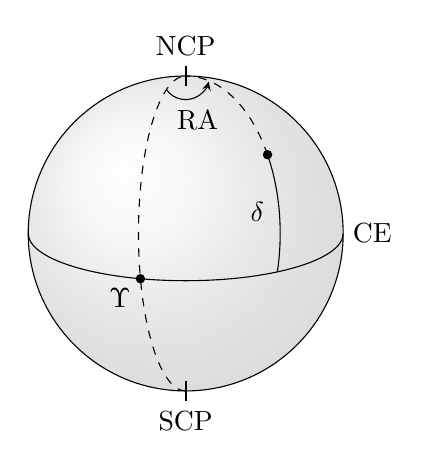
\begin{tikzpicture}[>=stealth]
            \shade[ball color=gray!40,opacity=0.2] (0,0) circle (2);
            \draw (0,0) circle (2);
            \draw[name path=ce] (-2,0) arc (180:360:2 and 0.6) node[right] {CE};
            \draw[dashed,rotate=90,name path=mer] (-2,0) arc (180:0:2 and 0.6);
            \draw[thick] (0, 1.875) -- (0, 2.125) node[above] {NCP};
            \draw[thick] (0, -1.875) -- (0, -2.125) node[below] {SCP};
            \draw[rotate=90] (300:2 and 1.2) arc (300:256:2 and 1.2) node[left=2pt,pos=0.5] {$\delta$};
            \draw[dashed,rotate=90] (300:2 and 1.2) arc (300:360:2 and 1.2);
            \fill[rotate=90] (300:2 and 1.2) circle (0.06);
            \draw[->] ([shift=(215:0.3)]0,2) arc (215:346:0.3) node[below left=7pt and -7pt] {RA};
            \fill[name intersections={of=ce and mer,by={X}},rotate=90] (X) circle (0.06) node[below left] {$\Upsilon$};
        \end{tikzpicture}
        \caption{Celestial Coordinates}
    \end{minipage}
    \begin{minipage}{0.45\textwidth}
        \centering
        \hspace{1cm}
        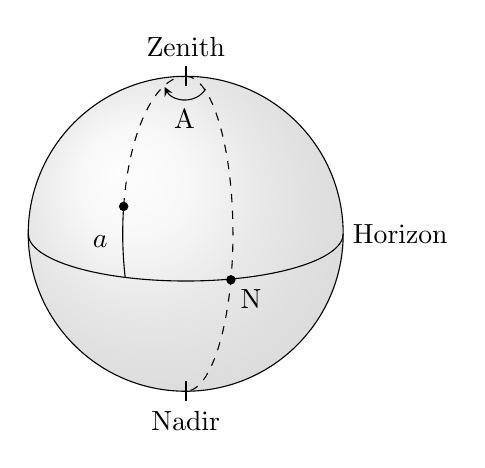
\begin{tikzpicture}
            \shade[ball color=gray!40,opacity=0.2] (0,0) circle (2);
            \draw (0,0) circle (2);
            \draw (-2,0) arc (180:360:2 and 0.6) node[right] {Horizon};
            \draw[dashed,rotate=-90] (-2,0) arc (180:0:2 and 0.6);
            \draw[thick] (0, 1.875) -- (0, 2.125) node[above] {Zenith};
            \draw[thick] (0, -1.875) -- (0, -2.125) node[below] {Nadir};
            \draw[rotate=-90] (260:2 and 0.8) arc (260:286:2 and 0.8) node[left=2pt,pos=0.5] {$a$};
            \draw[dashed,rotate=-90] (260:2 and 0.8) arc (260:180:2 and 0.8);
            \fill[rotate=-90] (260:2 and 0.8) circle (0.06);
            \draw[<-,>=stealth] ([shift=(207:0.3)]0,2) arc (207:327:0.3) node[below,pos=0.5] {A};
            \fill[rotate=-90] (73:2 and 0.6) circle (0.06) node[below right] {N};
        \end{tikzpicture}
        \caption{Horizontal Coordinates}
        \label{fig:alt_az_system}
    \end{minipage}
\end{figure}

Denoted $\Upsilon$ is the vernal equinox\footnote{This point is also known as the \textit{First Point of Aries}, although it has since moved into Pisces}, a reference point where $\delta = 0\degree$ and $\RA = 0\h$. The \textit{declination} ($\delta$) is considered within the principal range of $-90\degree \leq \delta \leq +90\degree$, and taken to be positive in the Northern hemisphere, and negative in the Southern hemisphere. The \textit{right ascension} increases rightwards from the arc of $0\h$ right ascension. If you've ever wondered why right ascension seems to increase leftwards while observing the night sky, it's because your perspective is from an observer on the `interior' of the sphere.

The horizontal coordinate system (or \textit{alt-az}) is similar, except the reference plane is the observer's horizon instead of the celestial equator. The pole directly above the observer is called the \textit{zenith}, and the one under the \textit{nadir}. The altitude ($a$) is positive measured upwards from the horizon, with the azimuth ($A$) measured \textbf{eastwards}\footnote{Azimuth can also be measured westwards or starting from cardinal South, but rarely in astronomy} from cardinal North. Cardinal points are nothing more than the NSEW directions on a compass.

\begin{Exercise}
Provided in the following table are the positions of celestial objects in Orion.

\setlength{\tabcolsep}{15pt}
\renewcommand{\arraystretch}{1.2}
\begin{tabular}{|c|c|c|c|c|c|}
    \hline
     & \textbf{Betelgeuse} & \textbf{Rigel} & \textbf{Tabit} & \textbf{M42} & \textbf{NGC2169} \\ \hline
    \textbf{Declination ($\delta$)} & $+\sexg{7}{24}{33}$ & $-\sexg{8}{10}{47}$ & $+\sexg{6}{59}{41}$ & $-\sexg{5}{26}{18}$ & $+\sexg{13}{56}{44}$ \\ \hline
    \textbf{Right Asc. ($\RA$)} & $\hms{5}{56}{16}$ & $\hms{5}{15}{30}$ & $\hms{4}{50}{56}$ & $\hms{5}{36}{23}$ & $\hms{6}{9}{33}$\\ \hline
\end{tabular}
\smallskip
\begin{enumerate}[label=(\roman*)]
    \item Calculate the distance between M42 and NGC2169.
    \item Solve entirely the spherical triangle made from the three stars.
\end{enumerate}
\end{Exercise}

\subsection{I got a B- for art}
Astronomy is largely based on observations. Unfortunately for us who have been cursed with clouds and skyglow, our observations are based on star charts and Stellarium. I've sunk too much time into astronomy to pivot to a more accessible hobby, so I like to turn off the lights and pretend that Stellarium is the night sky.

Ultimately, if you wish to answer questions such as when the Sun will rise, how long before a star will set, and how to convince yourself a 36cm f/2.2 telescope is a worthwhile investment, you will need to understand how to use the celestial sphere.

Notice the celestial sphere says nothing about the location of the observer. It only offers a standard of locating objects. We will need to combine it with the horizontal coordinate system in order to locate them relative to us.

\begin{figure}[h]
    \centering
    \begin{minipage}{0.45\textwidth}
        \centering
        \hspace{1cm}
        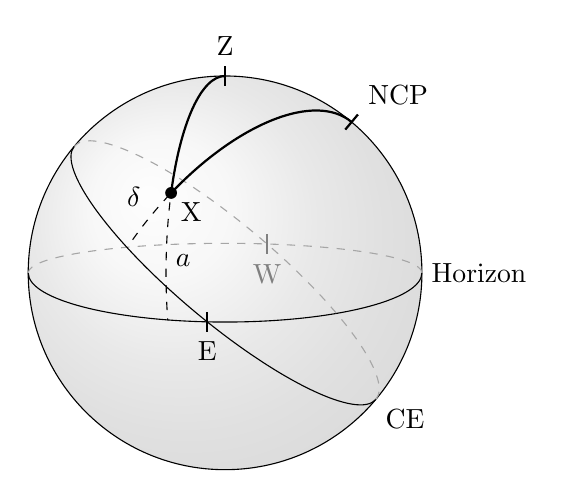
\begin{tikzpicture}[scale=1.25]
            \shade[ball color=gray!40,opacity=0.2] (0,0) circle (2);
            \draw (0,0) circle (2);
            \draw[thick] (0, 1.9) -- (0, 2.1) node[above] {Z};
            \draw[thick,rotate=-40] (0, 1.9) -- (0, 2.1) node[above right] {NCP};
            % Horizon
            \draw[name path=horz] (-2,0) arc (180:360:2 and 0.5) node[right] {Horizon};
            \draw[dashed,gray!70,rotate=180,name path=horzp] (-2,0) arc (180:360:2 and 0.3);
            % Celestial equator
            \draw[name path=ce,rotate=-40] (-2,0) arc (180:360:2 and 0.5) node[below right] {CE};
            \draw[dashed,gray!70,rotate=140,name path=cep] (-2,0) arc (180:360:2 and 0.5);
            \path[name intersections={of=horz and ce,by=E}];
            \draw[thick] ($(E)+(0,0.1)$) -- ($(E)-(0,0.1)$) node[below] {E};
            \path[name intersections={of=horzp and cep,by=W}];
            \draw[gray,thick] ($(W)+(0,0.1)$) -- ($(W)-(0,0.1)$) node[below] {W};
            % Declination
            \draw[name path=decp,thick,rotate=50] (2,0) arc (0:83:2 and 0.95);
            \draw[dashed,rotate=50] (83:2 and 0.95) arc (83:100:2 and 0.95) node[above left,pos=0.5] {$\delta$};
            % Altitude
            \draw[name path=altp,thick,rotate=90] (2,0) arc (0:67:2 and 0.6);
            \draw[dashed,rotate=90] (69:2 and 0.6) arc (69:104:2 and 0.6) node[right,pos=0.5] {$a$};
            % Object
            \fill[name intersections={of={decp and altp},by=X}] (X) circle (0.06) node [below right] {X};
        \end{tikzpicture}
    \end{minipage}
    \begin{minipage}{0.45\textwidth}
        \centering
        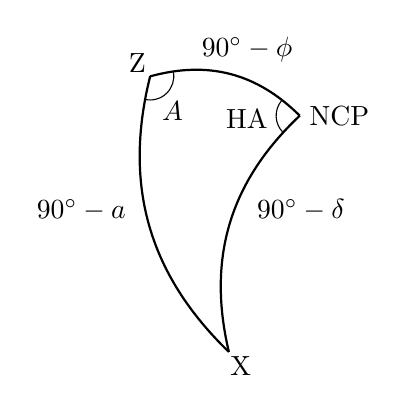
\begin{tikzpicture}
            \coordinate (A) at (-0.7, 1.7);
            \coordinate (B) at (1.2, 1.2);
            \coordinate (C) at (0.3, -1.8);
            \draw[thick] (A) to[bend left] (B) node[pos=0.5,above right=50pt and -5pt] {$90\degree - \phi$};
            \draw[thick] (B) to[bend right=30] (C) node[pos=0.8,right=15pt] {$90\degree - \delta$};
            \draw[thick] (A) to[bend right=30] (C) node[pos=0.5,left=25pt] {$90\degree - a$};
            \node[above left=-2pt and -2pt] at (A) {Z};
            \node[above right=-7pt and 0pt] at (B) {NCP};
            \node[below right=-2pt and -3pt] at (C) {X};
            \draw ([shift=(255:0.3)]A) arc (255:370:0.3) node[below left=7pt and -7pt] {$A$};
            \draw ([shift=(140:0.3)]B) arc (140:225:0.3) node[above left=-2pt and 2pt] {HA};
        \end{tikzpicture}
    \end{minipage}
    \medskip
    \label{fig:combined_coords}
    \caption{why didn't I draw these by hand I regret everything}
\end{figure}

The celestial equator and the horizon intersect at cardinal East and West (take a guess why). The \textit{meridian} is the half-great circle passing through cardinal North, the zenith, and cardinal South. The \textit{prime vertical} is the half-great circle passing through cardinal West, the zenith, and cardinal East. 

Do not be fooled into thinking that the prime meridian and prime vertical are absolute reference points because they have the same suffix. The meridian and prime vertical are relative to the observer. The prime meridian is the line of $\RA = \sexg{0}{}{}$. This is the devious work of astronomers before us with terrible nomenclature who are trying to get into your head.

We don't draw the vernal equinox here, because the observer's position alone isn't sufficient to determine its position. Like any other star, the vernal equinox is just another point in the constantly moving night sky. A constantly moving reference isn't very fun to work with, so in Fig.\;\ref{fig:combined_coords} we have done away with the right ascension. Instead, we opt for the related and more useful quantity the \textit{hour angle}:
\begin{equation}
    \HA = \left\{\ 
    \begin{matrix} 
        \text{Hours since crossing} \\ 
        \text{the meridian} 
    \end{matrix}
    \ \right\}
    = - \left\{\ 
    \begin{matrix} 
        \text{Hours to crossing} \\ 
        \text{the meridian} 
    \end{matrix}
    \ \right\}
    \label{eqn:ha_definition}
\end{equation}

An object's HA is essentially a 24-hour timer starting when the object crosses the meridian. The object is said to \textit{culminate} when it is right on the meridian with $\HA = \sexg{0}{}{}$. Hour angles are sometimes given in the negative to represent hours \textbf{until} crossing the meridian. 

Fun fact! The acronyms for A.M. and P.M are derived from the Latin phrases \textit{ante meridiem} and \textit{post meridiem}, meaning before and after midday. Here, \textit{meridiem} means midday, in the accusative singular form of the 5th declension root noun \textit{meridies}. Nevertheless, one can also interpret it as the portions of the day where the Sun is positioned before and after the meridian.

From the cosine law, we can also derive a form more convenient to work with:
\begin{equation}
\label{eqn:cosine_law_astro}
    \sin a = \sin \delta \sin \phi + \cos \delta \cos \phi \cos \HA
\end{equation}

\begin{Exercise}
You are contemplating existence atop a giant rubber duckie in the middle of the Great Pacific Garbage Patch ($\phi = \sexg{38}{2}{},\,\lambda = 147.8\degree$) when you spot Gemini rising.

\begin{enumerate}[label=(\roman*)]
    \item Which star, Castor or Pollux, rises first?
    \item How soon after does the other star culminate?
\end{enumerate}

Some undetermined amount of time later, you find yourself on another duck in the middle of the Australian outback ($\phi = -\sexg{26}{46}{},\,\lambda = \sexg{120}{20}{}$).

\begin{enumerate}[label=(\roman*)]
\setcounter{enumi}{2}
    \item Do the answers above hold?
\end{enumerate}

\setlength{\tabcolsep}{20pt}
\renewcommand{\arraystretch}{1.2}
\begin{center}
\begin{tabular}{|c|c|c|}
     \hline
     & \textbf{Castor} & \textbf{Pollux} \\ \hline
     \textbf{Declination ($\delta$)}& $+\sexg{31}{53}{17.79}$& $+\sexg{28}{1}{34.31}$ \\ \hline
     \textbf{Right Asc. ($\RA$)}& $\hms{7}{34}{35.86}$& $\hms{7}{45}{18.95}$ \\
     \hline
\end{tabular}
\end{center}
\end{Exercise}

\subsection{\texttt{a e s t h e t i c s}}

Even without light pollution, we wouldn't be able to see \textit{circumpolar} stars in Singapore, as we are much too close to the equator. These are stars that never set. In Fig.\;\ref{fig:star_trail}, notice how some stars trace out a complete circle. Conversely, there exist stars that never rise for an observer (which lack a name). The paths of these stars are small circles parallel to the celestial equator that never intersect with the horizon.

\begin{Exercise}
Find the condition(s) to be satisfied in order for a star to be circumpolar, or never rise. \\
Note: \textit{Don't memorize this - learn how to derive this from diagrams!}
\end{Exercise}
\begin{Answer}
    \begin{table}[h]
        \begin{tabular}{|l|l|l|}
        \hline
         & \textbf{Never setting} & \textbf{Never rising} \\ \hline
        \textbf{Northern Hemisphere} $(\phi > 0\degree)$ & $\delta > 90\degree - \phi$ & $\delta < \phi - 90\degree$ \\ \hline
        \textbf{Southern Hemisphere} $(\phi < 0\degree)$ & $\delta < -90\degree - \phi$ & $\delta > 90\degree + \phi$ \\ \hline
        \end{tabular}
    \end{table}
\end{Answer}

It is possible for the Sun to never rise or set within the day. This happens in the polar regions where it can be completely dark or always daytime for stretches of months at a time. This phenomenon only takes place on certain locations on Earth: either northwards of the Arctic circle or southwards of the Antarctic circle, the two lines of latitude at $\phi = 66.5\degree$ and $\phi = -66.5\degree$ respectively.

\begin{figure}[h]
    \centering
    \includegraphics[width=0.6\textwidth]{img/startrails.jpg}
    \caption{Imagine this in Singapore hahahaha}
    \label{fig:star_trail}
\end{figure}

To be pedantic, there is an \textit{upper} and \textit{lower} culmination since any object will cross the meridian twice within a sidereal day. There is little astronomical name-mangling here -- when the object is at its highest position in the sky, that's the upper culmination. For most objects, they set below the horizon, so the lower culmination is obscured by the ground. The ambiguity only sets in for circumpolar stars and the like, so we opt to drop the prefix most of the time.

\section{Time is a social construct}
It is now time for us to discuss the topic of timezones. Stars could not care less about the time, but we do. It is the folly of humanity to bind ourselves to the arbitrary concept of time, but we will have to make do. For us living in Singapore, we only have one timezone. We can be blissfully ignorant of timezone gymnastics unlike our Russian comrades with eleven\footnote{Interestingly, France has technically the most timezones at 12 because that counts their territories around the globe too.}.

Remember how the right ascension is measured relative to a reference of $\hms{0}{}{}$? Greenwich time operates essentially the same way. The prime meridian in this case refers to the Greenwich prime meridian\footnote{You might find references to the Paris prime meridian in some historical texts, but that was so last century.}, the line of longitude at $\lambda=0\degree$. The reference time on the prime meridian is denoted as the \textit{Greenwich mean time} (GMT). Usually, a timezone will also be given relative to GMT, e.g. Singapore Standard Time as SST (GMT+8).

Similar to the right ascension, places east and west of the prime meridian are \textbf{ahead} and \textbf{behind} GMT respectively, with every $15\degree$ corresponding to a change of $\hms{1}{}{}$ (Eqn.\;\ref{eqn:time_conversion}). 

The astute reader would have realized that with Singapore's longitude ($\lambda = 103.2198\degree$), we should comfortably be in GMT+7.

\begin{figure}[h]
    \centering
    \includegraphics[width=0.6\textwidth]{img/idl.jpg}
    \caption{Kiribati date line go brrrr}
    \label{fig:idl}
\end{figure}

For economic reasons, Singapore decided to move one hour ahead. I was not kidding when I said that anything to do with time is completely arbitrary. Just take a look at Kiribati in the +13/14 timezone (Fig.\;\ref{fig:idl}). How is that even allowed? The line that snakes around it is the International Date Line. 
Unlike the celestial coordinate system, our time systems have dates, and need to be able to make the distinction of when the day ends. No matter what day of the year, Alaska (GMT-10) will always be a day behind Kiribati (GMT+14).

\subsection{Times are tough}
Thanks to human interventions, what we see on clocks, the \textit{civil time}, is somewhat subjective and has little significance for astronomy. You could declare the land you stand on to be following the GMT+35 timezone and the stars wouldn't suddenly change. 

A better, more objective measurement of time is needed for astronomy. The Greenwich Mean Time is one such standard, and we will revisit it in depth later. While civil time timezones are chunked into integer hour offsets from GMT, the \textit{Local Mean Time} (LMT) is continuous and depends solely on the longitude of the location.

\begin{equation}
\label{eqn:greenwich_to_local}
    \mathrm{LMT} = \mathrm{GMT} + \Delta \tau
\end{equation}
\begin{equation}
    \Delta \tau = \frac{\lambda}{15^\mathrm{\degree/h}};\quad\lambda=
    \begin{cases}
        < 0,& \mathrm{westwards} \\
        > 0,& \mathrm{eastwards}
    \end{cases}
\end{equation}
There is a similar standard called the \textit{Greenwich Sidereal Time} (GST), and similarly from Eqn.\;\ref{eqn:greenwich_to_local}, the \textit{Local Sidereal Time} (LST).

The LST is defined with respect to the RA and the HA:
\begin{equation}
    \mathrm{LST} = \RA + \HA
\end{equation}
Together with Eqn.\;\ref{eqn:ha_definition}, we can see that the LST is \textbf{equal to the RA of any star currently on the meridian}. For GST, this corresponds to the prime meridian (the meridian of an observer at Greenwich). Conceptually, this time difference $\Delta \tau$ is due to the rotation of the Earth -- remember that the night sky isn't actually moving, but it is us who is doing the rotating.

\begin{Exercise}
Stranded on an island in the middle of the Pacific Ocean ($\phi=\sexg{5}{53}{1},\,\lambda=\sexg{162}{4}{42}$W), you get bored and decide to dig a hole in the ground. To your amazement, you unearth missing Inca treasure. Amongst them is a strange contraption that you figure out to be a clock that tells you when the Pleiades ($\RA=\hms{3}{47}{24},\,\delta=+\sexg{24}{07}{}$) rises, which ostensibly is in exactly 2 hours. Suddenly, you remember a promise to call your friend Noiro-san who works lives near Orion Happy Park ($\phi=\sexg{26}{35}{13},\,\lambda=\sexg{127}{59}{20.93}$E) when the Orion Nebula is about to culminate there. How long is it before you should call him?
\end{Exercise}
\begin{Answer}
\flipanswer{In $\hms{7}{10}{54}$}
\end{Answer}
\medskip

The difference between GST and GMT arises from the fact that a sidereal day is only $\hms{23}{56}{4}$ long. The GST at the same UT\footnote{We will be using UT and GMT interchangably. Refer to Appendix\;\ref{app:timesystems} for more details} tomorrow would be $3^\mathrm{m}56^\mathrm{s}$ \textbf{later}.

That is nice and simple, but to do any meaningful calculations, we still need to have a reference GST at some date and UT\footnote{Page B8 of the Astronomical Almanac gives a formula for this relative to J2000. Interesting, but probably not useful to you.}. Usually, this is given at $\hms{0}{}{}$ UT on 1st Jan of the year.

\begin{equation}
    \text{Current GST} = \left\{\ 
    \begin{matrix} 
        \text{Reference} \\ 
        \text{GST given}
    \end{matrix}
    \ \right\}
    + \left\{\ 
    \begin{matrix} 
        3^\mathrm{m}56^\mathrm{s} \text{ per day}\\
        \text{since reference \textbf{date}}
    \end{matrix}
    \ \right\}
    + \left\{\ 
    \begin{matrix} 
        \text{\textbf{UT difference} between} \\
        \text{current and reference}
    \end{matrix}
    \ \right\}
    \times \frac{3^\mathrm{m}56^\mathrm{s}}{\hms{24}{}{}}
\end{equation}

If you understand the concepts, this formula is pretty intuitive. The last two terms account for the fact that a sidereal day is shorter than 24 hours. The last term is similar to the second term, behaving as a scaling factor for the time difference.

\begin{Exercise}
In Singapore, we can't see the Large Magellanic Cloud ($\RA=\hms{5}{24}{},\,\delta=-\sexg{70}{}{}$) because we only see clouds (everywhere). Suppose you were in Phuket ($\phi=\sexg{7}{53}{},\,\lambda=\sexg{98}{24}{}$E), which follows the GMT+7 timezone. On which day of 2017 will the LMC culminate at 9pm? You are given that the Greenwich sidereal time at $\hms{0}{}{}$ UT on 1st January 2017 is around $\hms{6}{43}{}$.
\end{Exercise}
\begin{Answer}
\flipanswer{Around 32 days since 1st January, or 2nd February}
\end{Answer}

\section{Boring Star}
In the grand scheme of things, the Sun is actually a pretty normal, average, ordinary star. 

\subsection{Sun is fast}
It is, however, a very fast zoom zoom star. Other stars move very slowly relative to the celestial sphere, with Barnard's star having the largest proper motion at $10''$ per year. The Sun moves this much in less than a minute.

Unlike other stars, the declination and RA of the Sun change across the span of the year. The Earth's axial tilt, or \textit{obliquity}, is roughly $\epsilon = 23.5\degree$. As the Sun moves in a different plane to the celestial equator, the declination of the Sun changes as the Earth makes its way about its orbit. Similarly, the position of the Sun against the background of stars will change. During the vernal equinox, the Sun will be in line with the First Point of Aries. 

The variable declination of the Sun is responsible for the seasons (as observed within the Northern hemisphere). The equinoxes occur when the Sun is directly on the celestial equator ($\delta = 0\degree$), and the solstices on the Tropic of Cancer/Capricorn ($\delta = +23.5\degree$ and $\delta = -23.5\degree$ respectively). Together with the Arctic/Antarctic circle, these form the \textit{five major lines of latitude}.

\begin{figure}[h]
    \centering
    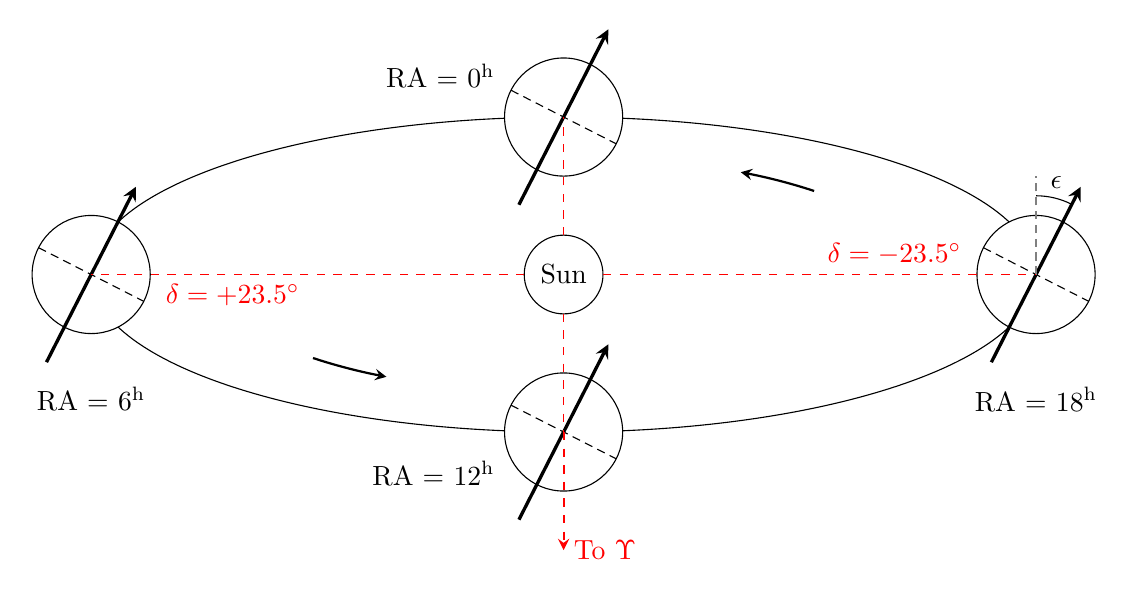
\begin{tikzpicture}[>=stealth]
        \def\TILT{27}
        %%
        \draw (0,0) circle (6 and 2);
        \draw (0,0) circle (0.5) node {Sun};
        % Winter Solstice
        \begin{scope}[shift=(0:6 and 2)]
            \draw[fill=white] (0,0) circle (0.75) node[below=1.3] {RA = $\hms{18}{}{}$};
            \draw[very thick,rotate=-\TILT,->] (0,-1.25) -- (0,1.25);
            \draw[densely dashed,rotate=-\TILT] (-0.75,0) -- (0.75,0);
            \draw[densely dashed,thick,gray] (0,0) -- (0,1.25);
            \draw ([shift=(90-\TILT:1)]0,0) arc (90-\TILT:90:1) node[pos=0.45,above] {$\epsilon$};
        \end{scope}
        % Summer Solstice
        \begin{scope}[shift=(180:6 and 2)]
            \draw[fill=white] (0,0) circle (0.75)  node[below=1.3] {RA = $\hms{6}{}{}$};
            \draw[very thick,rotate=-\TILT,->] (0,-1.25) -- (0,1.25);
            \draw[densely dashed,rotate=-\TILT] (-0.75,0) -- (0.75,0);
        \end{scope}
        % Vernal Equinox
        \begin{scope}[shift=(90:6 and 2)]
            \draw[fill=white] (0,0) circle (0.75)  node[above left=0.25 and 0.75] {RA = $\hms{0}{}{}$};
            \draw[very thick,rotate=-\TILT,->] (0,-1.25) -- (0,1.25);
            \draw[densely dashed,rotate=-\TILT] (-0.75,0) -- (0.75,0);
        \end{scope}
        % Autumnal Equinox
        \begin{scope}[shift=(270:6 and 2)]
            \draw[fill=white] (0,0) circle (0.75)  node[below left=0.25 and 0.75] {RA = $\hms{12}{}{}$};;
            \draw[very thick,rotate=-\TILT,->] (0,-1.25) -- (0,1.25);
            \draw[densely dashed,rotate=-\TILT] (-0.75,0) -- (0.75,0);
        \end{scope}
        % Lines
        \draw[red,dashed] (0.5,0) -- (0:6 and 2) node[above left,pos=0.85] {$\delta=-23.5\degree$};
        \draw[red,dashed] (0,0.5) -- (90:6 and 2);
        \draw[red,dashed] (-0.5,0) -- (180:6 and 2) node[below right,pos=0.85] {$\delta=+23.5\degree$};
        \draw[red,dashed] (0,-0.5) -- (270:6 and 2);
        % Direction
        \draw[thick,->] (45:4.5 and 1.5) arc (45:60:4.5 and 1.5);
        \draw[rotate=180,thick,->] (45:4.5 and 1.5) arc (45:60:4.5 and 1.5);
        % Vernal point
        \draw[red,->,thick,dashed] (270:6 and 2) -- (0,-3.5) node[right] {To $\Upsilon$};
    \end{tikzpicture}
    \caption{nyoom}
    \label{fig:sun_ra_dec}
\end{figure}

Sometimes, we will be required to interpolate the RA and declination of the Sun. Fortunately, this is nothing more than a sine curve (Fig.\;\ref{fig:declination_graph}).

\begin{figure}[h!]
    \centering
    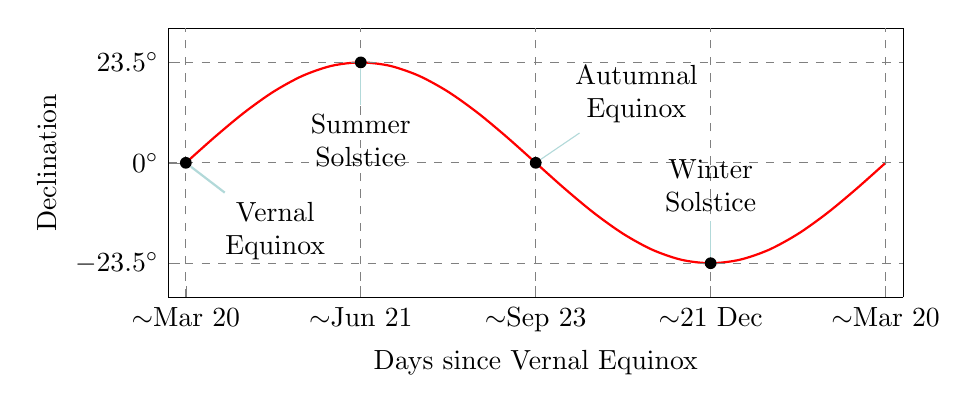
\begin{tikzpicture}
        \begin{axis}[
            width=0.9\textwidth,
            height=5cm,
            smooth,
            enlargelimits=0.025,
            axis x line*=top,
            axis y line*=right,
            xmajorticks=false,
            ymajorticks=false,
            xmin=0, xmax=365,
            ymin=-30, ymax=30
        ]
            \addplot[red,domain=0:365,thick] { 23.5 * sin(x*360/365) };
        \end{axis}
        \begin{axis}[
            width=0.9\textwidth,
            height=5cm,
            enlargelimits=0.025,
            axis x line*=bottom,
            axis y line*=left,
            xlabel={Days since Vernal Equinox},
            ylabel={Declination},
            xmin=0, xmax=24,
            ymin=-30, ymax=30,
            xtick={0, 6, 12, 18, 24},
            xticklabels={$\sim$Mar 20, $\sim$Jun 21, $\sim$Sep 23, $\sim$21 Dec, $\sim$Mar 20},
            ytick={-23.5,0,23.5},
            yticklabels={$-23.5\degree$, $0\degree$, $23.5\degree$},
            xmajorgrids=true,
            ymajorgrids=true,
            grid style={dashed,gray}
        ]
            \node[pin={[pin edge=thick,align=center]-45:{Vernal\\Equinox}},circle,fill,inner sep=1.5pt] at (axis cs:0,0) {};
            \node[pin={[align=center]-90:{Summer\\Solstice}},circle,fill,inner sep=1.5pt] at (axis cs:6,23.5) {};
            \node[pin={[align=center]45:{Autumnal\\Equinox}},circle,fill,inner sep=1.5pt] at (axis cs:12,0) {};
            \node[pin={[align=center]90:{Winter\\Solstice}},circle,fill,inner sep=1.5pt] at (axis cs:18,-23.5) {};
        \end{axis}
    \end{tikzpicture}
    \caption{Almost too easy}
    \label{fig:declination_graph}
\end{figure}

\subsection{Sun is appear}
Now that we can determine the RA and declination of the Sun, we can invoke the same calculations as for any other old star. Although the Sun's celestial coordinates changes from sunrise to sunset, unless otherwise stated, we will invoke the almighty approximation they remain \textbf{constant} within the day.

We can then derive the sunrise equation from Eqn.\;\ref{eqn:cosine_law_astro} by setting $a=0$:
\begin{equation}
    \cos \HA = -\tan \delta \tan \phi
\end{equation}
It might be called the sunrise equation, but evidently it works for sunset and whatever star of your choosing as well. But wait! By setting $a=0$, the catch is this equation gives the HA for when the \textbf{center} of the Sun is on the horizon. This is fine and dandy for stars which are taken as tiny point sources, but you might recall that the Sun appears as a humongous ball. Usually, sunrise is reckoned when the top of the solar disk (or the \textit{upper limb}) is on the horizon. Ain't it ironic how the sunrise equation is more useful for stars than the Sun?

\begin{Exercise}
You find yourself shipwrecked on an island again. Making a mental note to stop going on dodgy cruises, you encounter an inhabitant of the island wearing his tribal clothing of a Hawaiian shirt and sunglasses. Fortunately, he speaks impeccable English and tells you that this is the mysterious island of Nalaguraidhoo ($\phi=\sexg{3}{29}{2},\,\lambda=\sexg{72}{48}{1}$E). Wishing to get the most aesthetic shot for your Instagram, you want to find the optimal spot to capture the sunset. At noon time, your watch tells you the time is 7:19 am on the the 17th of October.
\begin{enumerate}[label=(\roman*)]
    \item According to your watch, when will the sunset start and end?
    \item What is the azimuth of the setting sun?
\end{enumerate}
\end{Exercise}
\medskip

\begin{figure}
    \centering
    \begin{minipage}[b]{0.45\textwidth}
        \centering
        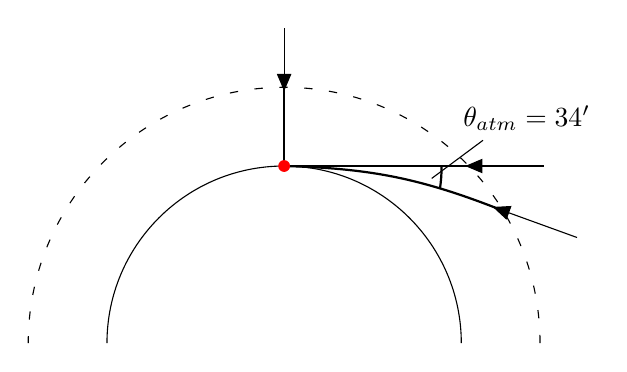
\begin{tikzpicture}[>=triangle 45]
            \draw (0:2.25) arc (0:180:2.25);
            \draw[loosely dashed] (0:3.25) arc (0:180:3.25);
            % \draw[thick] ([shift=(90:0.3)]0,2.25) arc (90:160:0.3) node[above left=0.2 and -0.2] {$z$};
            \draw[thick] (0,2.25) -- (2.35,2.25);
            \draw[<-] (2.3,2.25) -- (3.3,2.25);
            \draw[thick] (0,2.25) -- (0,3.25);
            \draw[<-] (0,3.2) -- (0,4);
            % \draw[thick] (0,2.25) -- (-1.558,2.852);
            % \draw[<-] (-1.558,2.852) -- (-2.491,3.213);
            \draw[thick] (0,2.25) to[bend left=10] (2.78,1.683);
            \draw[<-] (2.65,1.73) -- (3.72,1.342);
            \draw[thick] ([shift=(0:2)]0,2.25) arc (0:-8:2);
            \node[pin={[pin edge={black}]85:$\quad\theta_{atm}=34'$}] at (1.75,2.0) {};
            \fill[red] (0,2.25) circle (0.075);
        \end{tikzpicture}
        \caption{light is bendy}
        \label{fig:atm_refrac}
    \end{minipage}
    \begin{minipage}[b]{0.45\textwidth}
        \centering
        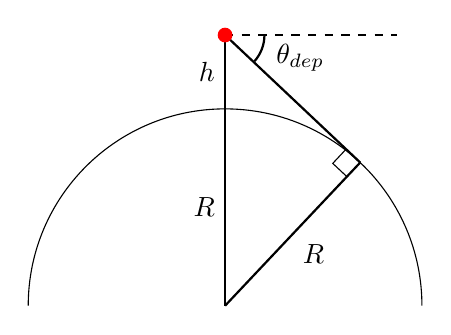
\begin{tikzpicture}[scale=1.25]
            \draw (0:2) arc (0:180:2);
            \draw[thick] (0,2) -- (0,2.75) node[left,pos=0.5] {$h$};
            \draw[thick] (0,0) -- (0,2) node[left=0,pos=0.5] {$R$};
            \draw[thick] (0,2.75) -- (1.373,1.455);
            \draw[thick] (0,0) -- (1.373,1.455) node[pos=0.5,below right=0 and 0] {$R$};
            \draw (1.238,1.311) -- (1.094,1.446) -- (1.229, 1.59);
            \draw[dashed] (0,2.75) -- (1.75,2.75);
            \draw[thick] ([shift=(0:0.4)]0,2.75) arc (0:-42:0.4) node[below right=-0.35 and 0.15] {$\theta_{dep}$};
            \fill[red] (0,2.75) circle (0.075);
        \end{tikzpicture}
        \caption{horizon is bendy}
        \label{fig:horz_depression}
    \end{minipage}
\end{figure}

There is also the effect of \textit{atmospheric refraction} (Fig.\;\ref{fig:atm_refrac}). Due to atmosphere not having a uniform density, incoming light undergoes a series of refractions, distorting and shifting the resultant image. Technically, we \textit{should} be considering this effect as long as we are doing terrestrial observations. We should also attempt to maintain any modicum of sanity we might have left, so in practice we don't. As with most things fluid, the atmosphere is terribly difficult to model, because it depends on various things such as the turbulent flow of air currents and temperature gradients. 

Generally, we will correct for this phenomenon only near the horizon, where it is much more pronounced. The \textbf{downwards} deflection is taken to be a constant value around $\theta_{atm} = 34'$.

There is also the effect of \textit{horizon depression} (Fig.\;\ref{fig:horz_depression}) which occurs when the observer is at an appreciably high elevation. The surrounding terrain is assumed to be near sea level -- usually the context will be the observer on the tip of a mountain or tall tower. The observer's effective horizon is the tangent line to Earth's surface, an angle $\theta_{dep}$ lower than the horizon at sea level:
\begin{equation}
    \theta_{dep} = \cos^{-1} \left( \frac{R}{R+h} \right)
\end{equation}

\begin{Exercise}
You have painstakingly climbed to the top of a mountain to commemerate the summer solstice. Deciding that a magnificent sight should be accompanied by a feast of burgers, you call for a delivery from MgRonalds with the frankly unreasonable request that it arrives right as the sun sets. However, the deliveryman arrives 4.1 minutes late, having calculated for the sunset as observed from the MgRonalds which is at sea level. If the mountain is situated at $\phi = 40\degree$, how high is the mountain you are on?
\end{Exercise}

\subsection{Inside you there are two Suns}
If you looked at Fig.\;\ref{fig:declination_graph} and thought: 
\begin{center}
    \textit{``Wow! Who would have thought the Sun's movement was so simple! The laws of physics governing the movement of the celestial bodies are truly magnificent to prescribe such wondrous elegance!''}
\end{center}

What did you expect? The Universe is a beautiful place and so is physics. Unfortunately, the Universe hates you and it has no qualms throwing rocks at you and laughing at your misery.

In reality, this curve will not be exactly a sine curve, unless Earth's orbit were perfectly circular. It does make our lives considerably easier, so we use it unless greater accuracy is desired.

The Sun we see in the sky, also known as the \textit{apparent Sun}, has changing velocity and declination. Earth's slightly eccentric orbit is problematic, as the Sun moves faster near perihelion and slower at aphelion. Making matters worse, the changing declination of the Sun (Fig.\,\ref{fig:sun_ra_dec}) means it traces a slightly different path across the sky everyday. 

Imagine having a clock with its hands moving at different speeds depending on the time of day. Maybe it decides to slow down only on Wednesdays but goes twice as fast on Fridays. What a terrible clock it would be! Fortunately, we have the concept of the \textit{mean Sun}, a fictitious body created with the sole purpose of being easier to work with. The mean Sun moves \textbf{along the celestial equator} at the average speed of the apparent Sun.

Some of you may be familiar with the GMAT, the Graduate Management Admission Test, which is for business and adminstration inclined people. But there is also another, for us astronomical folk, the \textit{Greenwich Mean Astronomical Time}. This GMAT is defined as the hour angle of the mean Sun, related to the GMT by \begin{align}
    \mathrm{GMT} &= 12\h - \HA_\mathrm{MS} \\
    &= 12\h + \mathrm{GMAT}
\end{align}
Essentially, the construct of a mean Sun is useful because it delivers a simple time standard, the \textit{mean solar time}. We have been using this synonymously with GMT, but this not be the case (refer to Appendix \ref{app:timesystems}).

A sundial uses the shadow cast by the position of the apparent Sun to tell the \textit{apparent solar time}, which is based on the hour angle of the apparent Sun.

To relate this to the mean solar time, we can use the \textit{equation of time}:
\begin{equation}
\label{eqn:eot}
    \EOT = \HA_\odot - \HA_\mathrm{MS}
\end{equation}
Some authors spit on this definition and throw it into the bin by switching the signs. Worry not, for we have the mnemonic \textbf{NYSS}\footnote{The word \textit{nyss} means \textit{just} or \textit{quite recently} in Swedish. I think you'll find that extremely useful}: New Year, Sun Slow. Regardless of the convention used, the apparent Sun lags behind the mean Sun, and this can be used to determine the sign of the EOT.

\begin{figure}[h!]
    \centering
    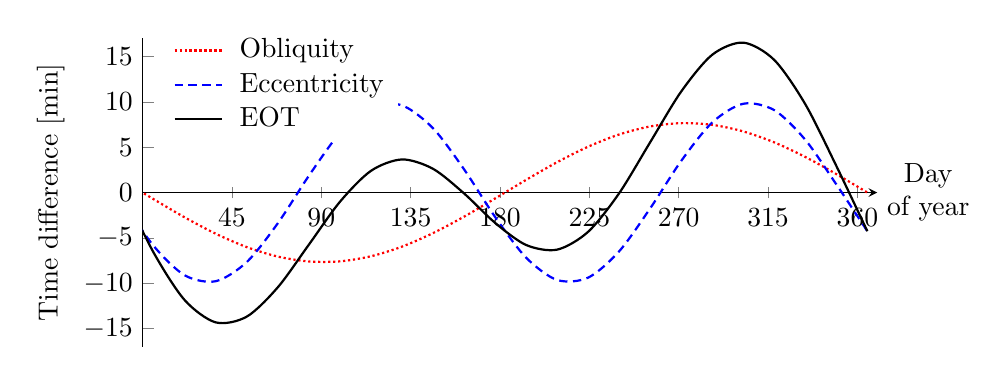
\begin{tikzpicture}
        \begin{axis}[
            width=0.9\textwidth,
            height=5.5cm,
            smooth,
            axis x line=middle,
            axis y line*=left,
            % enlarge x limits={abs=5},
            enlarge y limits={abs=2},
            xtick distance=45,
            ytick distance=5,
            xmin=0, xmax=370,
            ymin=-15, ymax=15,
            xlabel={Day\\of year},
            ylabel={Time difference [min]},
            xlabel style={align=center,at=(current axis.right of origin),anchor=west},
            legend cell align={left},
            legend style={draw=none,column sep=4,anchor=west,at={(0.03,0.85)}}
        ]
            \addplot[red,densely dotted,domain=-10:365,thick] { -7.655 * sin(x*360/365) };
            \addlegendentry{Obliquity}
            \addplot[blue,densely dashed,domain=-10:365,thick] { 9.873 * sin(x*720/365 + 3.588/6.283*360) };
            \addlegendentry{Eccentricity}
            \addplot[black,thick,domain=-10:365,thick] { (9.873 * sin(x*720/365 + (3.588/6.283*360))) - (7.655 * sin(x*360/365)) };
            \addlegendentry{EOT}
        \end{axis}
    \end{tikzpicture}
    \caption{even this is an approximation lmao}
    \label{fig:eot}
\end{figure}

For example, we can tell that Fig.\,\ref{fig:eot} uses the sign convention from Eqn.\,\ref{eqn:eot} since $\EOT > 0$ implies $\HA_\odot > \HA_{MS}$.

Although the difference in the declination of both Suns is also changing, we don't have to care about that yet -- we will see this soon in an interesting phenomenon that takes up its own chapter! Don't worry though, it's really fun\footnote{There are two ways to be fooled. One is to believe what isn't true; the other is to refuse to believe what is true. - Søren Kierkegaard}! When dealing with time, we are primarily concerned with the difference between their hour angles. 

The EOT is actually an approximation with its two major components being the obliquity and eccentricity of Earth's orbit. However, there are also secondary effects that contribute to the equation of time such as:
\begin{itemize}
    \item Precession of Earth's axis
    \item Nutation of Earth's axis
    \item Precession of the equinoxes
\end{itemize}
Unless you're doing some advanced astrodynamics, a quantitative formulation of these will never be required.

As a side note, when we talk about the local sidereal time, we actually mean the local \textbf{mean} sidereal time. The secondary effects outlined above also affects the apparent position of stars. Correspondingly, we have a local \textbf{apparent} sidereal time. You won't really see much of this so don't worry too much about it.

\section{To Be Continued (?)}

%\section{Analemmas}
If you were to look at the Sun at the same time every single day, you would have a good chance of permanent blindness. More importantly, you would have noticed that the Sun's position, even at the same exact time each day, changes in a peculiar manner.

Clearly, the Sun's celestial coordinates are different from other stars as it changes over the course of the year\footnote{The celestial coordinates of stars do change due to their proper motion, but are taken to be constant on short timescales}. We have seen how the apparent Sun has a declination that changes with the seasons (cf. Fig.\,\ref{fig:declination_graph}) as well as a variable right ascension (cf. Fig.\,\ref{fig:eot}).

The result is an aesthetic figure eight hanging in the sky:
\begin{figure}[h!]
    \centering
    \includegraphics[width=0.6\textwidth]{img/analemma.jpg}
    \caption{$\lim_{x->0^+} \frac{1}{x}$}
\end{figure}

The mean Sun is useful in visualizing the analemma as it acts as a reference point. In the blindness-inducing thought experiment outlined above, the position of the imaginary mean Sun remains fixed. This unsurprising result follows from the relationship between the mean solar time and UT. 

You could think of the analemma as a curve parameterized by time:
\begin{equation}
    \mathcal{C}(t) = \left\langle\, \RA_\odot(t) - \RA_\mathrm{MS}, \, \delta_\odot(t) - \delta_\mathrm{MS} \,\right\rangle
\end{equation}

For now, let us only concern ourselves with the shape of the analemma. To do so, it suffices to only care about the positions of the mean Sun and apparent Sun. The observer's location does not come into play just yet, so kindly temporarily forget about the horizontal coordinate system.

\subsection{\texttt{nasm -f elf analemma.asm}}
In this section, we will deconstruct and reassemble the analemma from its constituents. 

Although the curve of the analemma is technically embedded on the surface of the celestial sphere, unfortunately technology has only progressed to the point where I can embed links and not 3-D objects in a PDF. We will make do with a slightly distorted projection of the analemma on a 2-D surface.

\begin{figure}
    \centering
    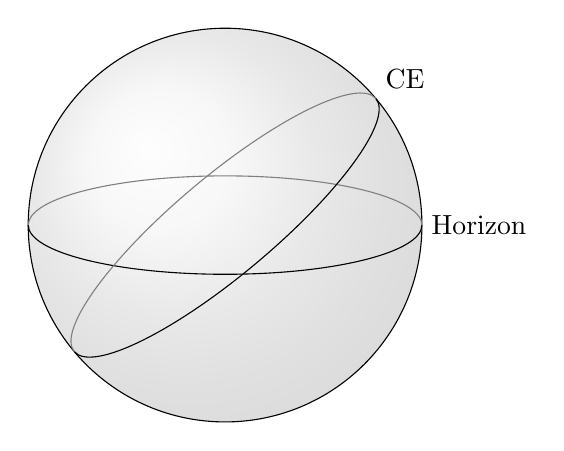
\begin{tikzpicture}[scale=1.25]
        \shade[ball color=gray!40,opacity=0.2] (0,0) circle (2);
        \draw (0,0) circle (2);
        % Horizon
        \draw[name path=horz] (-2,0) arc (180:360:2 and 0.5) node[right] {Horizon};
        \draw[gray] (-2,0) arc (180:0:2 and 0.5);
        % Celestial equator
        \draw[name path=ce,rotate=40] (-2,0) arc (180:360:2 and 0.5) node[above right] {CE};
        \draw[gray,rotate=40] (-2,0) arc (180:0:2 and 0.5);
    \end{tikzpicture}
    \caption{Caption}
    \label{fig:my_label}
\end{figure}

% vert is the declination sine curve
% horz is the eot (obliquity only)
% insert eccentricity (horz becomes EOT)
% wiki analemma highlights the left-right asymmetry (note the scale)


%%
%%  Appendices
%%
\appendix

\section{More things about time}
\label{app:timesystems}

\subsection{Disambiguation}

Colloquially, GMT can refer to either Universal Time (UT) or Coordinated Universal Time (UTC), which are entirely different in concept. This is a matter of loose definitions and even looser morals. UTC is based on atomic clocks, but due to manual corrections the difference is typically $<1^\mathrm{s}$.

Even when speaking of UT, it is an umbrella term referring to several standards. In common parlance, UT refers specifically to UT1, the successor to the older UT0 standard. Although they are both based on the mean solar time, it is terribly difficult to measure the Sun precisely. Instead, it is maintained by an assortment of measurements on satellites, the Moon and even quasars.

We can also note a distinction between UT and GMT should we argue semantics. They are used interchangeably, but GMT is a time \textit{zone}, while UT is a time \textit{standard}. Although we have used UT throughout these notes, GMT is actually based on UTC. Given the current time in UTC, you could calculate the time in UTC for a star to culminate. It would, however, be a conceptual faux pas to read a UTC time off a sundial, or when doing any calculations with the position of the Sun. For brevity and to spare you from the confusion, UTC is not used at all in these notes. 

\section{Derivations}
\label{app:derivations}

\subsection{Cotangent four-part formula}
In the event that you can't remember the formula, you can derive it from the other two spherical trigonometric laws. If you can't remember those either, then I wish you all the best.

The cotangent four-part formula is useful when specifically looking at 4 consecutive angles and sides, where we only have quantities of any 3 parts. The proof is also much cleaner when we take this into account.
\begin{figure}[h]
    \centering
    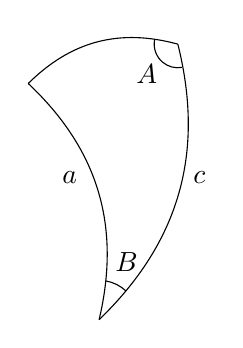
\begin{tikzpicture}
        \coordinate (A) at (0.7, 1.7);
        \coordinate (B) at (-1.2, 1.2);
        \coordinate (C) at (-0.3, -1.8);
        \draw (A) to[bend right] (B);
        \draw ([shift=(47:0.5)]C) arc (47:80:0.5) node[black,pos=0.5,above right=1pt and -4pt] {$B$};
        \draw ([shift=(170:0.3)]A) arc (170:280:0.3) node[black,pos=0.5,below left=-3pt] {$A$};
        \draw (B) to[bend left=30] (C) node[black,pos=0.5,left=13pt] {$a$};
        \draw (A) to[bend left=30] (C) node[black,pos=0.5,right=22pt] {$c$};
    \end{tikzpicture}
\end{figure}

Without loss of generality, let us assume we are dealing with the variables shown above. Using the two angles with their cosine laws:
\begin{gather}
    \cos a = \cos b \cos c + \sin b \sin c \cos A \\
    \cos b = \cos a \cos c + \sin a \sin c \cos B
\end{gather}

The variable $b$ is not in the final expression, so it can be substituted away to yield
\begin{equation}
    \cos a = \cos a \cos^2 c + \sin a \sin c \cos c \cos B + \cos A \,\frac{\sin B}{\sin A}\, \sin c 
\end{equation}

Simplifying and rearranging,
\begin{align}
\begin{split}
    \cos c \cos B + \cot A \sin B &= \frac{\cot a}{\sin c} \left( 1 - \cos^2 c \right) \\
    &= \cot a \sin c
\end{split}
\end{align}

The variables used here are for a generic spherical triangle. It can be converted to the form shown in Eqn.\,\ref{eqn:cotangent_four_part} using the substitutions:
\begin{equation*}
    \begin{split}
        A &\rightarrow \theta_o \\ 
        B &\rightarrow \theta_i
    \end{split}
    \qquad
    \begin{split}
        a &\rightarrow l_o \\
        c &\rightarrow l_i
    \end{split}
\end{equation*}

% TODO: spherical trickery
% declination from spherical triangle to sine curve
% draw right spherical triangle -> sine rule -> arcsin(sin wt sin e) \approx e sin wt
% rmb e should be in rad

% \section{Cool stuff}
% \subsection{Duals}
% \label{app:duals}
% In physics and mathematics, there is a very useful concept called a \textit{dual}. Say you have a mathematical object or concept, or generally a \textit{thing}, then $X*$ is the dual of $X$
% \begin{equation}
%     X^* = \mathcal{D}\{X\}
% \end{equation}
% such that the dual of the dual is the original \textit{thing} itself 
% \begin{equation}
%     \mathcal{D}\{X^*\} = (\mathcal{D}\circ\mathcal{D})\{X\} = X
% \end{equation}
% The dual is incredibly useful in parts of math and physics, as it is essentially the same \textit{thing} but viewed from another angle. As an illustration, say you have two sets $A$ and $B$:
% \begin{figure}[h!]
%     \centering
%     \begin{tikzpicture}
%         \draw (-0.75,0) circle (1.25) node[left=10pt] {$A$};
%         \draw (0.75,0) circle (1.25) node[right=10pt] {$B$};
%         \draw (-2.5, -1.75) -- (2.5, -1.75) -- (2.5, 1.75) -- (-2.5, 1.75) -- cycle node[left=3pt,pos=0.3] {$\xi$}; 
%     \end{tikzpicture}
% \end{figure}

% Let's say that you have a statement $S$ about these two sets, then its dual can be obtained by substituting in $S$: $\cap\rightarrow\cup$, $\cup\rightarrow\cap$, $\varnothing\rightarrow\xi$ and $\xi\rightarrow\varnothing$. For example:
% \begin{equation}
%     S\colon\, (A \cap B) \cup (A \cap \overline{B}) = A \quad \xrightarrow{\mathcal{\ D\ }} \quad S^*\colon\, (A \cup B) \cap (A \cup \overline{B}) = A
% \end{equation}
% \begin{equation}
%     S\colon\, (A \cap B) \cap (A \cap \overline{B}) = \varnothing \quad \xrightarrow{\mathcal{\ D\ }} \quad S^*\colon\, (A \cup B) \cup (A \cup \overline{B}) = \xi
% \end{equation}

% Of course the idea of a dual is more nuanced, but it's very complicated to explain such a general concept. As long as you get the vibe it's alright. You don't really need to understand this to use polar triangles.

%% something for counting days in a month
%% higher order effects (precession of the equinoxes/ earth's axis, nutation)

\end{document}